%\documentclass[journal]{vgtc}                % final (journal style)
\documentclass[review,journal]{vgtc}         % review (journal style)
%\documentclass[widereview]{vgtc}             % wide-spaced review
%\documentclass[preprint,journal]{vgtc}       % preprint (journal style)


\ifpdf%                                % if we use pdflatex
  \pdfoutput=1\relax                   % create PDFs from pdfLaTeX
  \pdfcompresslevel=9                  % PDF Compression
  \pdfoptionpdfminorversion=7          % create PDF 1.7
  \ExecuteOptions{pdftex}
  \usepackage{graphicx}                % allow us to embed graphics files
  \DeclareGraphicsExtensions{.pdf,.png,.jpg,.jpeg} % for pdflatex we expect .pdf, .png, or .jpg files
\else%                                 % else we use pure latex
  \ExecuteOptions{dvips}
  \usepackage{graphicx}                % allow us to embed graphics files
  \DeclareGraphicsExtensions{.eps}     % for pure latex we expect eps files
\fi%

%% it is recomended to use ``\autoref{sec:bla}'' instead of ``Fig.~\ref{sec:bla}''
\graphicspath{{figures/}{pictures/}{images/}{./}} % where to search for the images

\usepackage{microtype}                 % use micro-typography (slightly more compact, better to read)
\PassOptionsToPackage{warn}{textcomp}  % to address font issues with \textrightarrow
\usepackage{textcomp}                  % use better special symbols
\usepackage{mathptmx}                  % use matching math font
\usepackage{times}                     % we use Times as the main font
\renewcommand*\ttdefault{txtt}         % a nicer typewriter font
\usepackage{cite}                      % needed to automatically sort the references
\usepackage{tabu}                      % only used for the table example
\usepackage{booktabs}                  % only used for the table example

\onlineid{0}

%% declare the category of your paper, only shown in review mode
\vgtccategory{Research}
\vgtcpapertype{application/design study}

%% Paper title.
\title{A Study on a User-Controlled Radial Tour for Variable Importance in High-Dimensional Data}
\author{Nicholas Spyrison, Dianne Cook, Kim Marriott}
\authorfooter{
%% insert punctuation at end of each item
\item
 Monash University\\
Australia
\\nicholas.spyrison@monash.edu\\
ORCiD: 0000-0002-8417-0212.
\item
 Monash University\\
Australia
\\dicook@monash.edu\\
ORCiD: 0000-0002-3813-7155
\item
 Monash University\\
Australia
\\kim.marriott@monash.edu\\
ORCiD: 0000-0002-9813-0377
}

%other entries to be set up for journal
\shortauthortitle{Spyrison \MakeLowercase{\textit{et al.}}: Study on User-Controlled Radial Tour}

%% Abstract section.
\abstract{Principal component analysis is a long-standing go-to method for exploring multivariate data. The principal components are linear combinations of the original variables, ordered by descending variance. The first few components typically provide a good visual summary of the data. \emph{Tours} also make linear projections of the original variables but offer many different views, like examining the data from different directions. The grand tour shows a smooth sequence of projections as an animation following interpolations between random target bases. The manual radial tour rotates the selected variable's contribution into and out of a projection. This allows the importance of the variable to structure in the projection to be assessed. This work describes a mixed-design user study evaluating the radial tour's efficacy compared with principal component analysis and the grand tour. A supervised classification task is assigned to participants who evaluate variable attribution of the separation between two classes. Their accuracy in assigning the variable importance is measured across various factors. Data were collected from 108 crowdsourced participants, who performed two trials with each visual for 648 trials in total. Mixed model regression finds strong evidence that the radial tour results in a large increase in accuracy over the alternatives. Participants also reported a preference for the radial tour in comparison to the other two methods.
} % end of abstract

%% Keywords that describe your work. Will show as 'Index Terms' in journal
%% please capitalize first letter and insert punctuation after last keyword
\keywords{Multivariate data visualization, variable importance, radial tour, linear dimension reduction,}

%% ACM Computing Classification System (CCS). 
%% See <http://www.acm.org/class/1998/> for details.
%% The ``\CCScat'' command takes four arguments.
%% !!Decpricated; use: https://www.acm.org/publications/class-2012

\CCScatlist{ % not used in journal version
 \CCScat{10003120}{Human-centered computing}%
{}{};
 \CCScat{10003120.10003145.10011770}{Human-centered computing}{Visualization design and evaluation methods}{}
}

% %% A teaser figure can be included as follows
% \teaser{
%   \centering
%   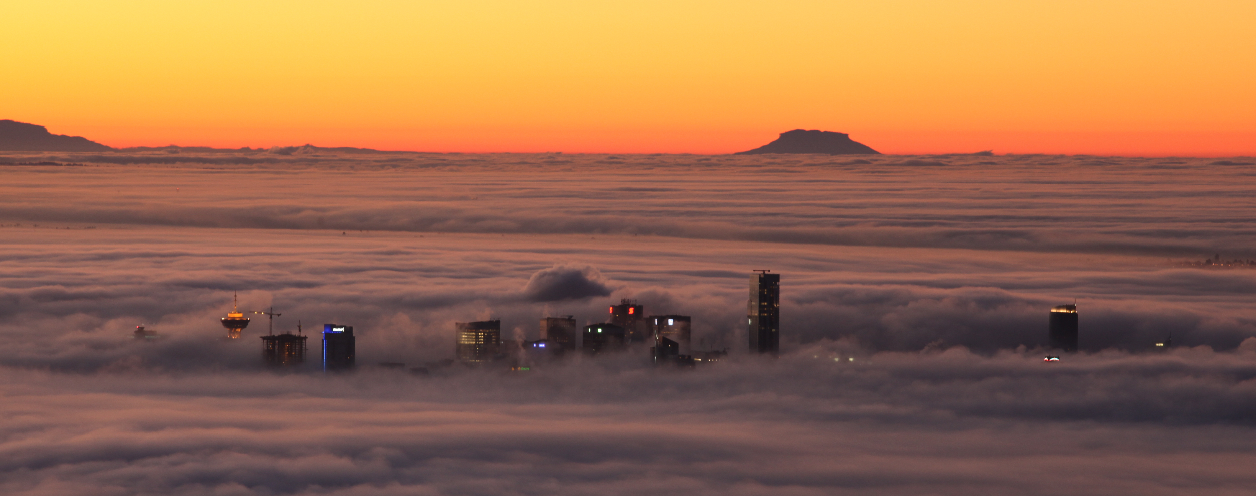
\includegraphics[width=\linewidth]{CypressView}
%   \caption{In the Clouds: Vancouver from Cypress Mountain. Note that the teaser may not be wider than the abstract block.}
%   \label{fig:teaser}
% }

%% Uncomment below to disable the manuscript note
%\renewcommand{\manuscriptnotetxt}{}

%% Copyright space is enabled by default as required by guidelines.
%% It is disabled by the 'review' option or via the following command:
% \nocopyrightspace


\vgtcinsertpkg

%%%%%%%%%%%%%%%%%%%%%%%%%%%%%%%%%%%%%%%%%%%%%%%%%%%%%%%%%%%%%%%%
%%%%%%%%%%%%%%%%%%%%%% START OF THE PAPER %%%%%%%%%%%%%%%%%%%%%%
%%%%%%%%%%%%%%%%%%%%%%%%%%%%%%%%%%%%%%%%%%%%%%%%%%%%%%%%%%%%%%%%%

\begin{document}

\firstsection{Introduction}

\maketitle


% 
% \hypertarget{introduction}{%
% \section{Introduction}\label{introduction}}

Despite decades of research, multivariate data continues to provide fascinating challenges for visualization. Data visualization is important because it is a key element of exploratory data analysis \cite{tukey_exploratory_1977} for assessing model assumptions and as a cross-check on numerical summarization \cite{anscombe_graphs_1973, matejka_same_2017, yanai_hypothesis_2020}. One challenge is measuring if a new technique yields a more informed perception of information than current practices.

Dimension reduction is commonly used with visualization to provide informative low-dimensional summaries of quantitative multivariate data. Principal component analysis (PCA) \cite{pearson_liii._1901} is one of the first methods ever developed, and it remains very popular. Visualization of PCA is typically in the form of static scatterplots of a few leading components. When the scatterplot is accompanied by a visual representation of the basis they are called a biplot \cite{gabriel_biplot_1971}. A basis is a \(p \times d\) matrix of the linear combination of the \(p\) variables mapped to a smaller \(d\)-dimensional space. That is, it is an orthogonal rotation matrix, the magnitude, and the angle that the variables contribute.

Dynamic visualizations called \emph{tours} \cite{asimov_grand_1985} animate through a sequence of linear projections (orthonormal bases). Instead of a static view, tours provide a smoothly changing view by interpolating between bases. There are various types of tours distinguished by how the paths are generated. Asimov originally animated between randomly selected bases in the \emph{grand} tour. The \emph{manual} tour \cite{cook_manual_1997} allows for user control over the basis changes. A selected variable (or component) can be rotated into or out of view or to a particular value. The \emph{radial tour} \cite{spyrison_spinifex_2020} is a variant of the manual tour that fixes the contribution angle and changes the magnitude along the radius. The permanence of the data points from basis to basis holds information between intermediate interpolated projections, and the user control of the basis could plausibly lead to more information being perceived than a static display. This is a hypothesis that a user study could assess.

Empirical studies have rarely assessed tours. An exception is \cite{nelson_xgobi_1999}, who compares scatterplots of grand tours on 2D monitors with 3D (stereoscopic, not head-mounted) over \(n=15\) participants. Participants perform cluster detection, dimensionality estimation, and radial sparseness tasks on six-dimensional data. They find that stereoscopic 3D leads to more accuracy in cluster identification, though the time to interact with the display was much higher in the 3D environment. In this work, we extend the evaluation of tours which compares the radial tour as benchmarked against the grand tour and discrete pairs of principal components.

The contribution of this paper is an empirical user study comparing the radial tour against PCA and the grand tour for assessing variable attribution on clustered data. This is the first empirical evaluation of the radial or manual tour. We discuss how this fits with other multivariate data visualization techniques and coordinated views of linear projections.

We are particularly interested in assessing the effectiveness of the new radial tour relative to common practice with PCA and grand tour. The user influence over a basis, uniquely available in the radial tour, is crucial to testing variable sensitivity to the structure visible in projection. If the contribution of a variable is reduced and the feature disappears, then we say that the variable was sensitive to that structure. For example, \autoref{fig:figClSep} shows two projections of simulated data. Panel (a) has identified the separation between the two clusters. The contributions in panel (b) show no such cluster separation. The former has a large contribution of V2 in the direction of separation, while it is negligible in the right frame. Because of this, we say that V2 is sensitive to the separation of the clusters.

\begin{figure*}

{\centering 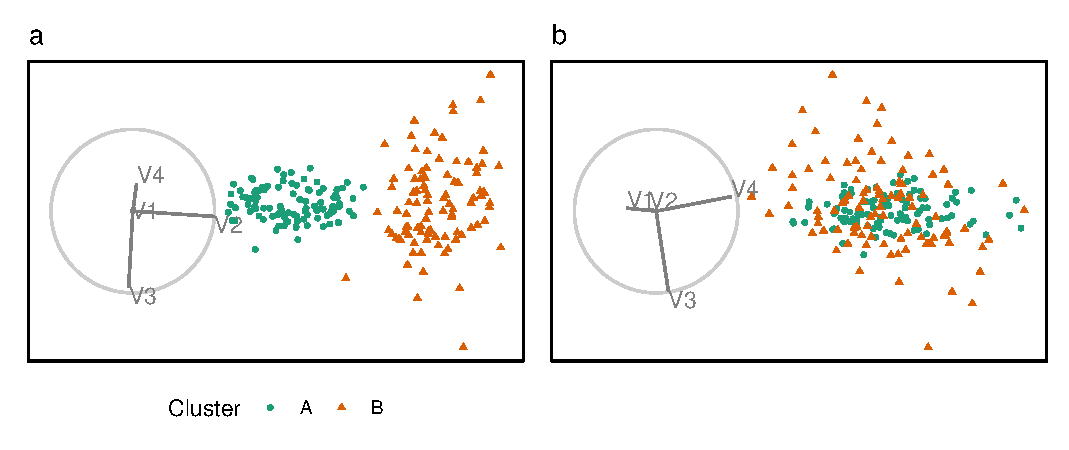
\includegraphics[width=1\linewidth]{./figures/figClSep} 

}

\caption{Illustration of cluster separation affected by variable importance. Panel (a) is a projection mostly of V2 and V3, and the separation between clusters is in the direction of V2, not V3. This suggests V2 is important for clustering, but V3 is not. Panel (b) shows a projection of mostly V3 and V4, with no contribution from V2 and little from V3. That there is no separation between the clusters indicates that V3 and V4 are not important.}\label{fig:figClSep}
\end{figure*}

Variable sensitivity is important for the interpretation of machine learning models. They are the magnitude and direction of contribution to the model. It is important that developers maintain the interpretability of models. Exploratory Artificial Intelligence (XAI) \cite{adadi_peeking_2018, arrieta_explainable_2020}, is an emerging field that extends the interpretability of such black-box models. Multivariate data visualization is essential for exploring feature spaces and communicating interpretations of models \cite{biecek_dalex_2018, biecek_explanatory_2021, wickham_visualizing_2015}.

The paper is structured as follows. Section \autoref{sec:relatedwork} provides background on standard visualization methods and linear dimension reduction techniques. Section \autoref{sec:userstudy} describes the experimental factors, task, and accuracy measure used. The results of the study are discussed in Section \autoref{sec:results}. Conclusions and potential future directions are discussed in Section \autoref{sec:conclusion}. More results, participant demographics, and analysis of the response time are available in the Supplemental Materials.


%%---CONTINUE WORK HERE---

%% if specified like this the section will be committed in review mode
\acknowledgments{
The authors wish to thank A, B, and C. This work was supported in part by
a grant from XYZ (\# 12345-67890).}

%\bibliographystyle{abbrv}
\bibliographystyle{abbrv-doi}
%\bibliographystyle{abbrv-doi-narrow}
%\bibliographystyle{abbrv-doi-hyperref}
%\bibliographystyle{abbrv-doi-hyperref-narrow}

\bibliography{spyrison-cook-marriott}
\end{document}

